\documentclass[a4paper,10pt]{article}
\usepackage[utf8]{inputenc}
\usepackage[spanish]{babel}
\usepackage{color}
\usepackage{graphicx}
\usepackage{todonotes}
\graphicspath{ {src/} }

\newcommand{\red}[1]{\textcolor{red}{#1}}
\newcommand{\tdn}[1]{\todo[inline]{#1}}

%opening
\title{Topic 1: Internet architecture and addressing}
\author{Albert Ribes}

\begin{document}

\maketitle

\begin{abstract}
\begin{itemize}
  \item Las respuestas en \red{rojo} son las que me hago persolnales para entenderlas bien.

  \item Las respuestas oficiales están normal
\end{itemize}
\end{abstract}

% \section
\listoftodos
\begin{enumerate}
  %1
  \item \textbf{Explica el rol y misión que tienen los RIR en la arquitectura de Internet. Indica cuantos y
que RIR’s operan. Explica el rol que tienen los LIR en la arquitectura de Internet. Indica que
relación hay entre un AS (Autonomous System) y un RIR y entre un AS y un LIR.}

\red{
RIR: Regional Internet Registry. Son las 5 redes que hay en el mundo: ARIN, LACNIC, AFRINIC, RIPE APNIC. Agrupan a los sistemas autónomos (AS). Son organizaciones independientes que apoyan la coordinación de recursos de Internet en una zona geográfica y desarrollan políticas consistentes y promocionan las buenas prácticas en Internet
}

\red{
LIR: Local Internet Registry. Son los miembros de los RIR. Los RIR distribuyen el espacio de direcciones IP a las LIR, y son estas últimas las que lo distribuyen a los usuarios finales.
}

\red{
Una NIR sería una National Internet Registry. Coordina las direcciones IP a nivel nacional. No hay ninguna en Europa, pero sí que hay en APNIC y LACNIC
}

\red{
Se puede considerar un AS a cualquiera que use el protocolo BGP. Puesto que dentro de una RIR se habla con BGP, todos los miembros han de usar BGP, y por lo tanto todos los miembros de un RIR son AS
}




  %2
  \item \textbf{A partir de la figura siguiente, explica la arquitectura de Internet y los distintos elementos
que participan en dicha arquitectura, así como, el modelo general de negocio de dicha arquitectura}

(La figura \ref{p2})

\tdn{Me da palo explicarlo, pero más o menos lo sé. Queda por hacer}

\begin{figure}[bh]
\centering
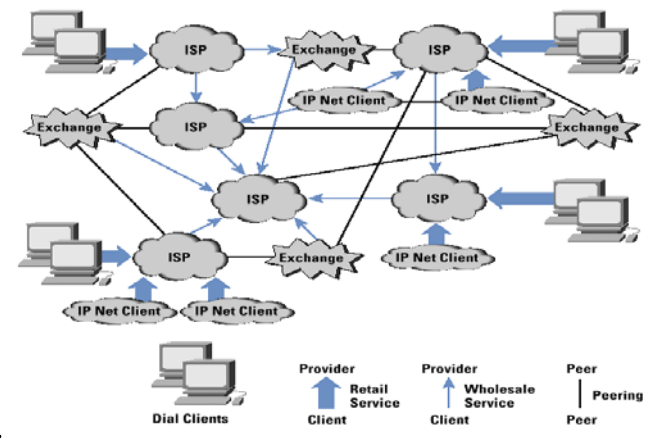
\includegraphics[width=8cm]{p2}
\label{p2}
\caption{}
\end{figure}

\red{En Internet hay organismos que proveen servicios, otros que consumen servicios y otros que actuan de intermediarios entre los dos}

\red{Para poder ofrecer servicios es necesario ser un sistema autónomo, y }

\red{Los elementos que participan en Internet son redes corporativas, dial-ups y sistemas autónomos (AS). }
  %3
  \item \textbf{Explica para que sirve una CDN (Content Distribution Network) y explica su
funcionamiento.}

\red{Una CDN es una plataforma de servidores distribuidos a lo largo de una zona geográfica que tiene el objetivo de facilitar la distribución de contenidos}

\red{La idea es que tener un único servidor para ofrecer un servicio presenta algunos problemas cuando son muchos los clientes que quieren consumir ese servicio. El primero es que ese servidor podría tener que soportar picos de peticiones a horas punta, y se podría saturar. Otro problema es que con un solo servidor no puedes estar cerca de todo el mundo, solo de unos pocos. Finalmente, si falla ese servidor todo el mundo se queda sin el servicio}

\red{En una CDN, muchos servidores distribuidos en distintos sitios tienen una cache con los servicios de un servidor central. Cuando un cliente quiere acceder a un servicio, se le asigna un servidor que está óptimamente localizado y con capacidad para soportar esa petición. Si ya ha accedido alguien a ese servicio en ese servidor, y el servicio no ha cambiado desde entonces, el servidor ya se ha guardado en la cache ese servicio, y puede ofrecerlo sin necesidad de que el servidor central participe. De esta manera toda la carga se distribuye entre todos los servidores y los clientes están más cerca geográficamente del servicio, con lo que es más rápido}


  %4
  \item \textbf{Explica que es un punto neutro y quien lo compone. Explica que es la matriz de peering
de un punto neutro.¿Qué condiciones hay que cumplir para ser miembro de un punto neutro?}

\red{Un punto neutro es un sistema para optimizar las comunicaciones entre distintos ISPs. Si no hay puntos neutros, cada par de ISPs que quieren establecer una relación deben tirar cable de uno hasta otro, y eso es muy costoso}

\red{Un punto neutro es un sitio al que pueden conectarse varios ISPs para establecer relaciones entre todos los otros que estén conectados. De esta manera se ahora en cable.}

\red{Un punto neutro lo componen los ISPs que están conectados a él.}

\red{La matriz de pearing de un punto neutro es una matriz que para cada par de ISPs que están conectados a él indica qué relación de peering tienen establecida}

\red{Cada punto neutro tiene sus propias normas, y por lo tanto establece sus propias condiciones para ser miembro}

  %5
  \item \textbf{Define que es un SLA (Service Level Agreement). Indica aquellos parámetros que
normalmente pueden formar parte de un SLA. ¿Qué ocurre si el ISP no cumple con alguno de los
parámetros que aparecen en el SLA? ¿Y si es el usuario o red corporativa?}

\red{Es el acuerdo que se define cuando 2 ISPs establecen una relación de peering y que penaliza al ISP que no cumple su contrato}

\red{Normalmente forma parte de un LSA:}
\red{
\begin{itemize}
  \item El porcentaje de tiempo que un ISP puede estar sin conexión
  \item El ancho de banda contratado
  \item El throughput
  \item El tiempo de respuesta en caso de fallo de conectividad
  \item La redundancia
  \item La seguridad
  \item La monitorización
  \item La calidad del servicio
\end{itemize}
}
\red{Si un ISP no cumple uno de los parámetros el precio a pagarle al siguiente mes será menor del acordado}

\red{Creo que un usuario o red corporativa pueden contratar distintos tipos de cosas, con alta y con baja fiabilidad. Si tienes la baja viabilidad y algo va mal, te fastidias}

  %6
  \item \textbf{Explica que representa el Cono de Clientes (“Customer Cone”) respecto a las direcciones
IPv4 y los AS y para que se utiliza. Ilústralo con un ejemplo. ¿Qué diferencia hay entre el cono de
clientes de un AS y su grado en la representación mediante un grafo donde los vértices son los
AS’s y las aristas son las relaciones entre AS’s?}

\red{El customer cone de un sistema autónomo es el conjunto de todos los sistemas autónomos y direcciones IP a las que se puede acceder desde él siguiendo únicamente los enlaces de sus clientes, de forma recursiva}

\red{Se utiliza para definir un ranking entre todos los sistemas autónomos}

\red{La diferencia es que la cantidad de vértices no ilustra correctamente la importancia que tienes, pues puedes tener un solo a otro ISP, pero que ese tenga muchos vértices}

  %7
  \item \textbf{Define e indica que representa el cono de clientes (“Customer Cone”) respecto a las
direcciones IPv4 y los AS. Dibuja una nueva figura respecto a la figura de abajo, con el nuevo
cono de clientes si (i) A y B (A es proveedor de B) cambian su relación a “A y B tienen una relación
de peer to peer”, (ii) A y B (A es proveedor de B) cambian su relación a “B es proveedor de A”.
Indica cual es el ``peering cone size ratio'' para el AS B en el caso de la figura y en los casos (i) y (ii).}

\tdn{Me da mucho palo hacer esto y se parece bastante a la anterior. Ya lo veremos}

  %8
  \item \textbf{¿Qué es un Sistema Autónomo (AS)? ¿Qué diferencia hay entre usar inter-domain e intra-domain routing en un AS? Explica los tipos de relaciones que tienen los AS’s.}

  \red{Un sistema autónomo es cualquier sistema que utilice el protocolo BGP}

  \red{Para hacer inter-domain routing es obligatorio usar BGP, pues es la única forma de identificarse}

  \red{Para hacer interdomain routing puedes hacerlo usando solamente IP}

  \red{Las relaciones que tienen entre ASs son:}

  \red{
  \begin{itemize}
    \item Proveedor a cliente:
    \item Cliente a proveedor
    \item Peer-to-peer con tránsito:
    \item Peer-to-peer sin tránsito:
  \end{itemize}
  }
  \tdn{Habría que explicar lo que es cada una de las relaciones}

  %9
  \item \textbf{En una relación BGP, ¿Qué rutas anuncia un ISP cliente a su proveedor?, ¿Y el proveedor a
su cliente? ¿Y de par a par de transito? ¿Y de par a par de no-transito?}

  %10
  \item \textbf{Explica las diferencias entre las direcciones PA (Provider Aggregatable) y PI (Provider
Independent). ¿Qué ventaja desde el punto de vista de encaminamiento proporciona
el uso de direcciones PA a los ISP’s?. ¿Puede un RIR asignar redes IPv4 /22 del tipo
PI?. Justifica tu respuesta.}

  %11
  \item \textbf{Explica como funciona el mecanismo de opciones de IPv6. Explica justificadamente si
es mas eficiente usar IPv6 en un router que usar IPv4}
\end{enumerate}

\end{document}
